% Created 2022-10-21 Fri 18:49
% Intended LaTeX compiler: pdflatex
\documentclass[hidelinks,11pt]{article}
\usepackage[utf8]{inputenc}
\usepackage[T1]{fontenc}
\usepackage{graphicx}
\usepackage{longtable}
\usepackage{wrapfig}
\usepackage{rotating}
\usepackage[normalem]{ulem}
\usepackage{amsmath}
\usepackage{amssymb}
\usepackage{capt-of}
\usepackage{hyperref}
\usepackage{caption}
\usepackage{subcaption} % sufigures facilities
\usepackage{float} % for H option
\usepackage{xcolor} % for the textcolor command
\usepackage[a4paper,width=150mm,top=25mm,bottom=25mm]{geometry} % fixes margins
\usepackage{changepage}
\author{Marcelo Veloso Maciel}
\date{}
\title{Working Paper}
\hypersetup{
 pdfauthor={Marcelo Veloso Maciel},
 pdftitle={W4 Essay},
 pdfkeywords={},
 pdfsubject={},
 pdfcreator={Emacs 28.2 (Org mode 9.6)},
 pdflang={English}}
\usepackage[authordate,strict,backend=biber,
bibencoding=inputenc]{biblatex-chicago}

\addbibresource{refs.bib}
\begin{document}

\maketitle

% parencite for indirect citation, textcite for direct citation

\section{Introduction}
The rise of polarization, the specter of democratic backsliding, and more
generally an apprehension with the survival prospects of democratic polities
have led to a renewed interest in what institutions mitigate vs. instigate
destabilizing dynamics, or that increase the adaptability of the political
system vis-{\'a}-vis both internal and external stressors
\parencite{Bednare2113843118, przeworski2019crises, chiopris2021wolf, ,
  tarko2014institutional}. Given their centrality to the input-output between
society and the state, electoral institutions naturally figure among the set of
such institutions under scrutiny \parencite{Wange2021systems}, and a strand of
the literature on collective choice has wondered whether the current electoral
victories of divisive candidates have not been an effect of informationally poor
decision procedures \parencite{potthoff2021condorcet, kurrild2018trump,
  woon2020trump}. This paper shows, however, that in 2018 presidential election
in Brazil, a highly polarized one, the election of a polarizing candidate, Jair
Messias Bolsonaro, was not simply an artifact of the decision procedure.
However, neither would he have won under any reasonable voting method. We
uncover partial conflicts between traditional stances regarding those methods.

Despite the multiple historical contingencies that might explain his victory,
one might naturally wonder what role the electoral system has had in it. After
all, it is well-known that the outcome of collective choices is fundamentally
dependent on the voting procedure \parencite{riker1982liberalism}. As Brazil's
majority with run-off system, most electoral systems use merely the first index
of the voters' preference rankings \parencite{grofman04_if_you_like_alter_vote}.
How would he have fared under informationally richer voting procedures, such as
pairwise comparison methods and positional voting procedures? Was he, and
arguably another democratically elected destabilizing candidate, a product of
decision procedures that favor divisive candidates over more inclusive ones
\parencite{igersheim22_compar_votin_method}? Would the result have changed with
a different set of candidates?

To answer those questions, I use a pre-electoral representative survey to
reconstruct the full 4-top rankings of the Brazilian population. Subsequently, I
use this augmented data to simulate the electoral results under the Borda and
Condorcet procedures and simulate the result for all positional procedures in
the top 4 and 3 candidate sets. Finally, I discuss the significance of the
results and conclude by pointing out the limitations of the endeavor.



\section{Theory}
There are multiple ways in which electoral institutions affect the Polity. Even
if we restrict our attention to a single rule, the aggregation procedure that
transforms ballots into a choice of a candidate \parencite{Goodin_2006}, two
perspectives of analysis ensue: static and dynamic. From a static point of view,
the decision procedures respect differing criteria such as monotonicity,
neutrality, anonymity, manipulability, and so on \parencite{nurmi1999voting}.
From a dynamic point of view, politicians and voters continuously adapt to the
rule in a system of feedback between the state and society
\parencite{Wange2021systems}. In this article, I'll focus on two ways a decision
procedure might reinforce destabilizing dynamics: by electing polarizing
candidates and by electing candidates with weak mandates.

\Big{\textcolor{red}{TODO}}: here talk more about the relationship between mandate and the positive
%% responsiveness

A polarizing or divisive candidate has strong support at the top
choice of voters, but also has a high share of bottom choices among the
electorate \parencite{igersheim22_compar_votin_method}.
The notion of a mandate of a candidate lets us situate both methods vis-{\`a}-vis
the one-choice informational environment typical of large-scale majoritarian
elections. At a minimum, a candidate has a mandate as long as it has won
under the voting procedure. A candidate has more mandate, however, the more significant
the difference between its vote share or score vs. the second most well-voted
candidate.


The destabilizing effects of electing divisive candidates or candidates with
weak mandates are well-documented in the literature
\parencite{kaminski2015empirical, luhrmann2018democracy, Baldassarrie2116863118,
  Bednare2113843118}. The paper focuses on the effect of decision procedures on
that phenomenon. But why would, after all, voting procedures have such effect?
For both a weak mandate and a polarizing candidate in the same example, suppose
there are 11 voters with preference A > B > C > D, 10 voters with B > C > D > A,
10 voters with C > B > D > A, 10 voters with D > B > C > A. A is naturally the
plurality winner, even though it was only the electorate's top choice of
\(27\%\) and was the bottom choice of the rest. It would lose in pairwise
comparisons to all other alternatives. In this example, the alternative to win
in all such pairwise comparisons would be B, a Condorcet Winner (CW). If we
assigned weights \((3,2,1,0)\) to positions in the ranking and summed the
scores, B would again be the winner, in this case, the Borda Winner (BW).


Note that being a CW is an even more robust notion of having a mandate. If the
candidate is a CW, then it would have won under all possible majority pairwise
comparisons against the other candidates. The BW lends itself to a similar
interpretation. Suppose a candidate wins under a voting procedure that only uses
the top choice of the electorate but is neither a BW nor a CW. In that case, it
has less mandate, in this generalized majoritarian perspective, than if it is
both, which signals a comprehensive social basis. In the former case, a
candidate who wins under the current voting procedure, but is neither a BW nor a
CW could be considered an artifact of the procedure. In the latter case, on the
other hand, the procedure would be just ``tracking'' a broader pattern of
support for the alternative.


This notion of mandate can be strengthened in the case of the Borda Count. The
Borda count can be seen as one method within a family of methods that assign
weights to positions in the ballot. In one extreme, the plurality voting method
assigns a score 1 to the top choice and 0 to all others. On the other extreme is
the antiplurality voting method, which assigns 1 to all positions besides the
last one. Between the two extremes are all possible ways of assigning a score to
the ballots of the electorate. The higher the proportion of positional voting
systems that the candidate would have won had the election used it, what
\textcite{tabarrok2001president} has called positional stability, the higher the
mandate of the candidate.

Note that both notions, CW and BW, require broader informational input from
voters (their full ranking) while outputting a result, in principle, more robust
to divisiveness (since rejection is taken into account) and more refined in
terms of mandate (since we have moved from simply winning to winning either in
all pairwise comparisons or even in most or all possible positional voting
procedures). This broader informational backdrop underlies current research on
the case of the United States and Donald Trump's electoral victory. Regardless
of the specificities of each paper all presuppose that the informational paucity
of only focusing on top choices blinds the States' socio-technical translation
of popular support into political input (the choice of candidate). For instance,
\textcite{potthoff2021condorcet, woon2020trump, kurrild2018trump} debate whether
Donald Trump was a CW in the primaries, with recommendations of
voting procedures that better track what the CW is, after all.
\textcite{igersheim22_compar_votin_method} goes a step further: they argue that
not only was Trump neither, but Sanders was the actual Borda and Condorcet
Winner, and generally the ``best'' candidate, if by best one understand a
candidate being the most inclusive and winning under the most alternative
decision procedures. We will see, however, that no such conclusion can be drawn
in the Brazilian case.

\section{Case/Data}

Jair Messias Bolsonaro was elected the president of Brazil in 2018. For more
than 20 years as a congressman, he was primarily a low clergy politician
defending the interests of the military and local police forces of the state of
Rio de Janeiro. The 2018 electoral scenario in Brazil was one of high rejection
of the traditional political elite, particularly of the Labour Party (Partido
dos Trabalhadores - PT), after corruption scandals and an impeachment process of
the previous president, Dilma Roussef, a Labor politician.


The main contestants,
among 13, were him, a rightist candidate; Fernando Haddad, a leftist candidate
from PT; Geraldo Alckmin, a center-right candidate; and Ciro Gomes, a
center-left candidate. The presidential election in Brazil follows a two-round
system. In the first round, \(8.79\%\) of the votes were White/Null, which means
the voting procedure does not count them. The result of the valid votes was the
following: Bolsonaro:Haddad:Ciro:Alckmin:Others =
\(46.3:29.28:12.47:4.76:7.19 \). Among the 9 other candidates, the highest vote
share was Jo{\~a}o Amo{\^e}do's with \(2.5\%\). All others got less than \(1\%\).
Moreover, There was a \(20\%\) abstention. In the second round, the result was:
Bolsonaro:Haddad = \(55.12\% : 44.78\% \). White/Null votes were \(9.57\%\) of
the total electorate. The abstention in this round was \(21.3\%\).

It is relevant to notice that the 2018 election was marked by two events. First,
the main leftist candidate,Lula, was prevented from running. He was arrested in
the beginning of the electoral campaigns, the process was deemed suspicious in
2021 since the judge\footnote{Bolsonaro nominated this judge Minister of
  Justice.} was cooperating with the prosecutor, and he won in 2022, in a
electoral process marked by irregularities in favor of Bolsonaro. The
distribution of support for Lula was markedly different from Haddad, who was
merely his replacement.

\Big{\textcolor{red}{TODO}} Elaborate on that!!!!

Second, in 09/06/2018, a month before the first round, there was an
assassination attempt against Bolsonaro. The knife attack most likely changed
the pattern of support for him.


The dataset used for the analysis is a representative street survey done on
10/02/2018, less than a week before the first round (10/07/2018). DataFolha did
this survey, an independent research institute highly esteemed and trusted by
Brazilian experts\footnote{I had access to the survey data, code-book, and
  questionnaire by creating an account and requesting access to them, available
  for educational/research purposes, at \url{https://www.cesop.unicamp.br}.}.
One question, in particular, is the only variable in our analysis: pairwise
comparisons between the 4 top candidates. With it is possible to reconstruct the
full 4-top ranking of the voter. Preliminary pre-processing has led me to drop
171 observations where all pairwise comparisons were missing and 132 in which
they were cyclic. This leaves us with 2937 out of 3240 observations. As
Table~\ref{Tab:Tcpairwise} shows only 1797 observations compared all 4
candidates. As such, we have to augment the data with transitive closures for
1140 observations by methods discussed in the next section.

\begin{table}[]\centering
\resizebox{0.5\columnwidth}{!}{
\begin{tabular}{|l|r|}
\hline
Number of Pairwise Comparisons & Frequency \\ \hline
1                    & 15        \\ \hline
2                    & 42        \\ \hline
3                    & 462       \\ \hline
4                    & 118       \\ \hline
5                    & 503       \\ \hline
6                    & 1797      \\ \hline
\end{tabular}
}
\caption{Frequency of pairwise comparisons in the dataset.}

\label{Tab:Tcpairwise}
\end{table}


\section{Methods}


After the rankings are inferred, I compute the Borda Count and Condorcet
Procedure for the top 4 candidates, calculate the victory scenarios for all
positional voting methods, and visualize the results for 3 candidates using
Saari's representation triangles \parencite{saari2012geometry}.

Saari's representation triangles provide a way of visualizing all possible
positional voting results of an election\footnote{For a complete exposition of
  this method see \textcite{saari1995basic} or \textcite{nurmi2002voting}.}.
Consider Figure \ref{fig:saari_nurmi}. The closer to a vertex, the better the
vertex's position in the social ranking. Region 1 corresponds to the social
ranking of \(A > B > C\), while Region 4 corresponds to the social ranking of
\(C>B>A\). The lines separating the regions represent indifference. The point in
which all lines meet corresponds to \(A \sim B \sim C\), while the line
separating Region 1 and 2 would correspond to \(A > B \sim C\). The three dots
are the results for the antiplurality, the borda and the plurality voting
methods. The line connecting the antiplurality and plurality results, the
extremes, denotes all possible positional results, including the result for the
Borda Count. The Borda Count point is always closer to the antiplurality result.
In this example, most positional voting methods would have agreed with the
plurality procedure outcome of \(B\) as the winner.

\begin{figure}[H]
 \centering
 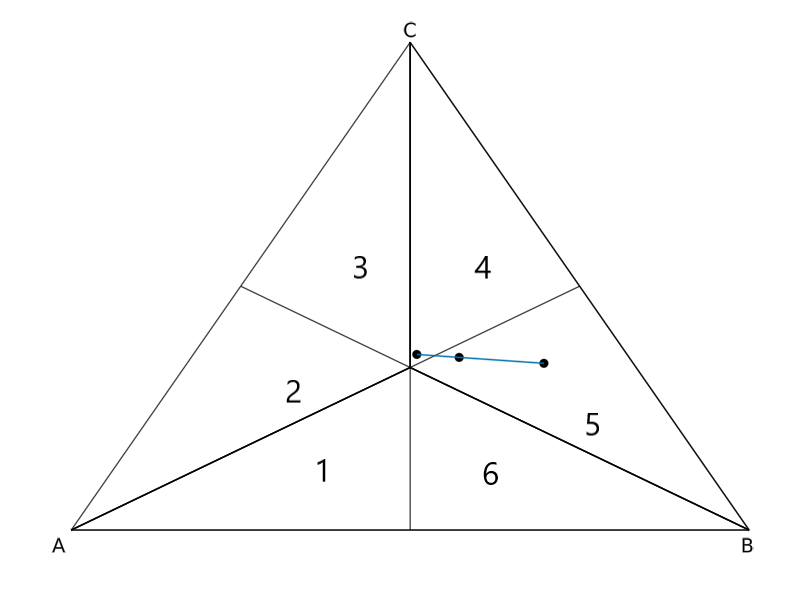
\includegraphics[width=0.8\columnwidth,
 height=0.3\textheight]{./images/simpletriangle.png}
 \caption{Saari representation triangle}
 \label{fig:saari_nurmi}
\end{figure}

To calculate all positional voting victories I use two facts proved by Donald
Saari \parencite{saari2012geometry, saari2001chaotic}: first, any positional
voting method for 4 candidates can be seen as assigning weights to rank
positions in a standardized manner \((1,s_{1},s_{2},0)\), where
\(0 \leq s_{2} \leq s_{1} \leq 1\); second, all such procedures will lie in the
convex hull of the plurality, antiplurality and vote for two procedures, with
respective weights of \((1,0,0,0), (1,1,1,0), (1,1,0,0)\). Calculating scenarios
amounts, thus, to vary the values of \(s_{1}\) and \(s_{2}\).

A further complication is a mismatch between the survey's plurality result and
the actual result of the first round. This is typical in surveys and might be
due to strategic voting, social desirability bias (not wanting to be seen as
``polarized''), or systematic refusal of part of the electorate to answer the
survey. Any imputation technique will reproduce this top-choice discrepancy.
Thus I'll show directly the mismatch between the imputation and the actual
vote. I ran the imputation algorithm on the top 4
candidates, which means that in the sample the \(7.19\%\) that voted for others
is kept constant. The result after applying the algorithm is
Bolsonaro:Haddad:Ciro:Alckmin:Others = \(36.7.7\% : 17.3\% : 14.1\% :7.19\% \).
Thus, Bolsonaro and Haddad are undervoted in the sample, while Ciro and Alckmin
are overvoted\footnote{Remember the actual result was
  Bolsonaro:Haddad:Ciro:Alckmin:Others = \(46.3:29.28:12.47:4.76:7.19 \).}. If
we were transferring the top choices from over-voted to under-voted, we could
simply transfer Alckmin \(\rightarrow\) Bolsonaro and Ciro \(\rightarrow\)
Haddad. However, there are 24 permutations of the top 4 candidates, with 6 for
each candidate in which they are the top alternative, which gives leeway to many
possible transfers.

If we are to transfer from Alckmin to Bolsonaro, we are lead to the problem of
first picking which ranking at the source should be chosen then which ranking at
the target should receive votes, while respecting how much the source has in
excess and how much the target needs. A natural sorting of which ranking should
be the source is the position of Bolsonaro in the ranking. We start with
rankings in which he is in the second position ((Alckmin, Bolsonaro, Ciro,
Haddad), (Alckmin, Bolsonaro, Haddad, Ciro)), then third position ((Alckmin,
Ciro, Bolsonaro, Haddad), (Alckmin, Haddad, Bolsonaro, Ciro )), then last
position ((Alckmin, Ciro, Haddad, Bolsonaro), ((Alckmin, Haddad, Ciro,
Bolsonaro))). Suppose we picked a source ranking from the first sorted rankings
set. What should be the target ranking among the rankings which have Bolsonaro
as the first choice? I transfer to the ranking that has minimal Kemeny's
distance to the source ranking \parencite{nurmi2002voting}. The Kemeny distance
counts the number of transpositions (switching of pairs) needed to go from one
permutation to another permutation. Thus, I transfer from the source ranking
the min(number of votes the source ranking has, the total number of votes the
under-voted needs, the total number of votes the over-voted can give). We update
the source ranking frequency, the target ranking frequency, the total number of
votes the under-voted needs, and the total number of votes the over-voted can
give. If the under-voted does not need any other votes we stop and go to another
over-voted \(\to\) under-voted transfer. If not we check if the over-voted can
still transfer votes to the current target under-voted. If yes we pick another
source ranking in the sorted rankings sets and repeat until either the source
has run out of votes it can give or the target has received enough votes. If not
we go to another over-voted \(\to\) under-voted transfer. In the end, this leads
to 24 possible transfer sequences from over-voted to under-voted. One possible
sequence is Alckmin \(\to\) Bolsonaro, then Alckmin \(\to\) Haddad, then Ciro
\(\to\) Haddad, then Ciro \(\to\) Bolsonaro. Another possible sequence is
Alckmin \(\to\) Bolsonaro, then Alckmin \(\to\) Haddad, then Ciro \(\to\)
Bolsonaro, then Ciro \(\to\) Haddad. This leads to 6 transfers that minimize the
euclidean distance between the inferred plurality result and actual result of
the first round. The result is invariant between them, so I only report the analysis for one of them.
\Big{\textcolor{red}{TODO}} Double check that!!!!!
The new inferred proportion now is:
Bolsonaro:Haddad:Ciro:Alckmin:Others = \(46.19:29.32:12.51:4.77:7.19 \).

\section{Results}
The inferred rankings are shown in Figure \ref{fig:rep_ot} and summarized in
Figure \ref{fig:counts}. Indeed, the candidates that went to the second round
were the most divisive ones. Among the more inclusive candidates, Ciro has more
second choices than third choices, while Alckmin is practically equilibrated
between those two. Moreover, Ciro has more first choices and less last choices
than Alckmin. There is also a relevant distinction among the divisive
candidates: Haddad's rejection was higher than his top-choice support, while the
opposite held for Bolsonaro. Those within-group, inclusive and divisive,
distinctions will be relevant to understand how each candidate fares against the
others.

\begin{figure}[H]
  \centering
  \begin{subfigure}[b]{0.49\textwidth}
    \centering
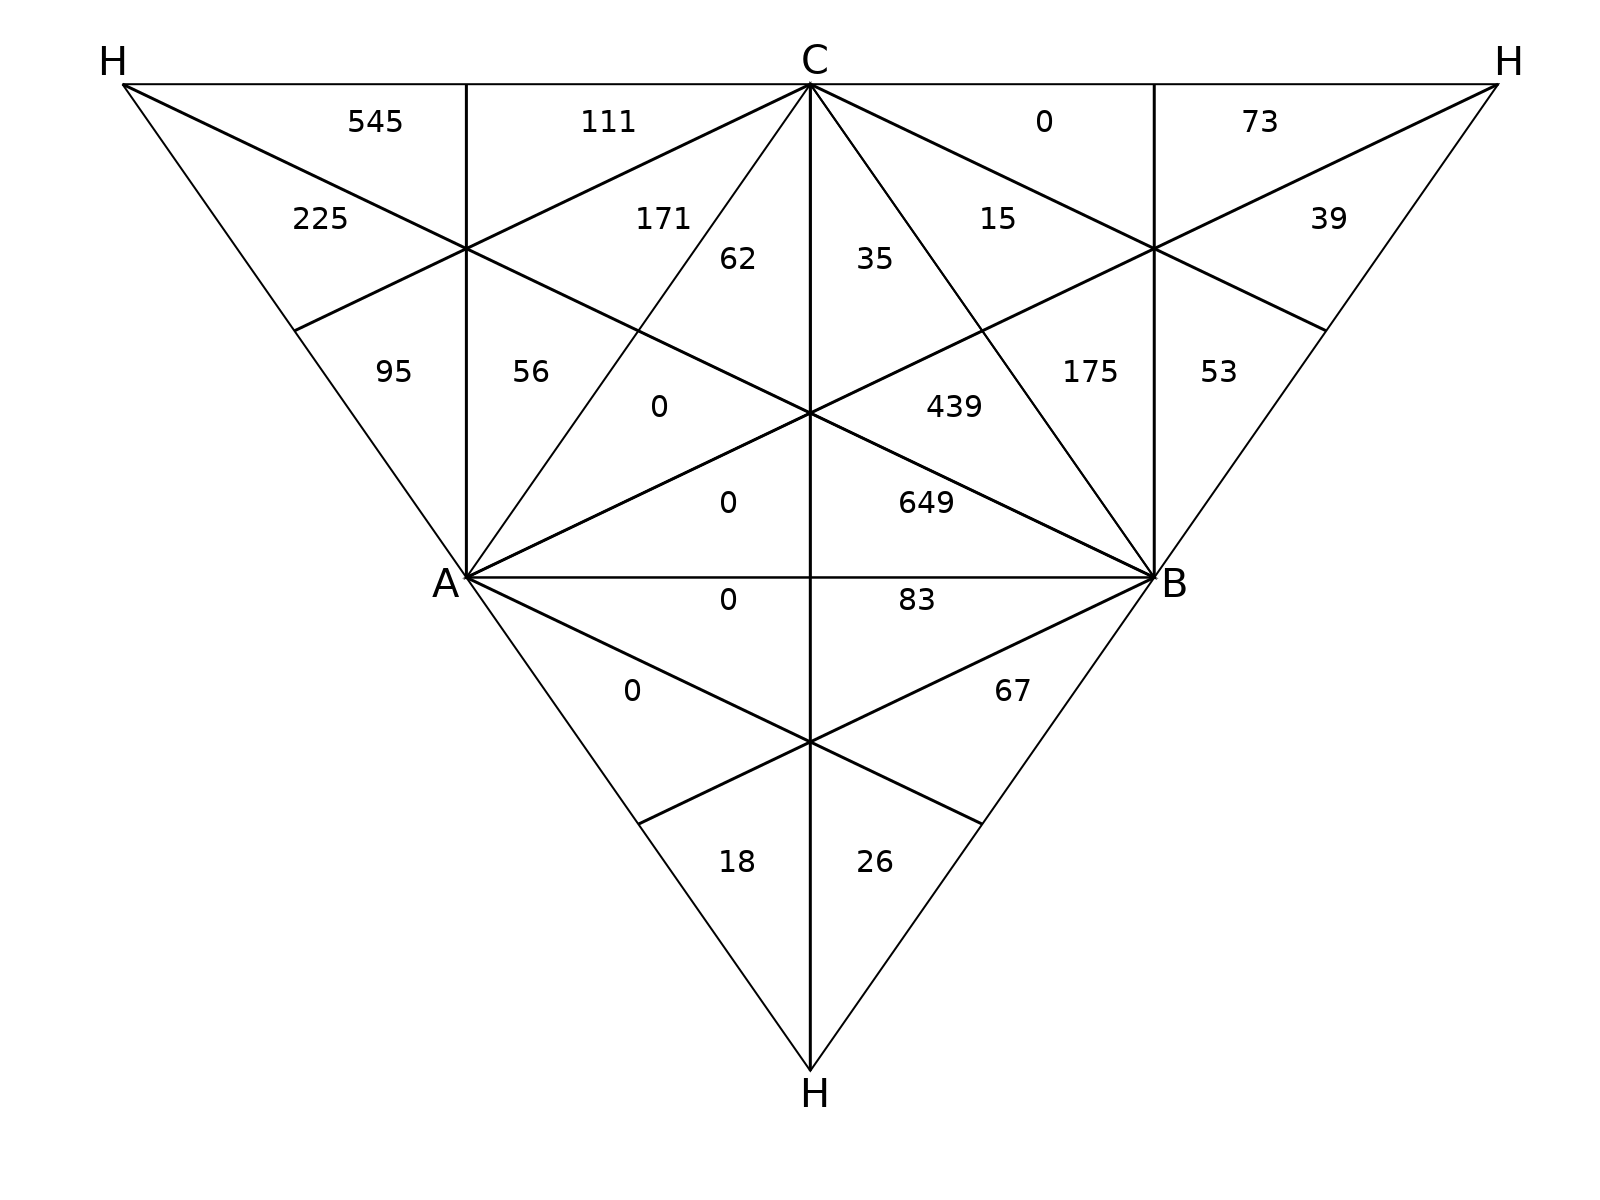
\includegraphics[width=\textwidth]{./images/representation_tetrahedron.png}
 \caption{Representation Tetrahedron}
 \label{fig:rep_ot}
\end{subfigure}
  \hfill
  \begin{subfigure}[b]{0.49\textwidth}
    \centering
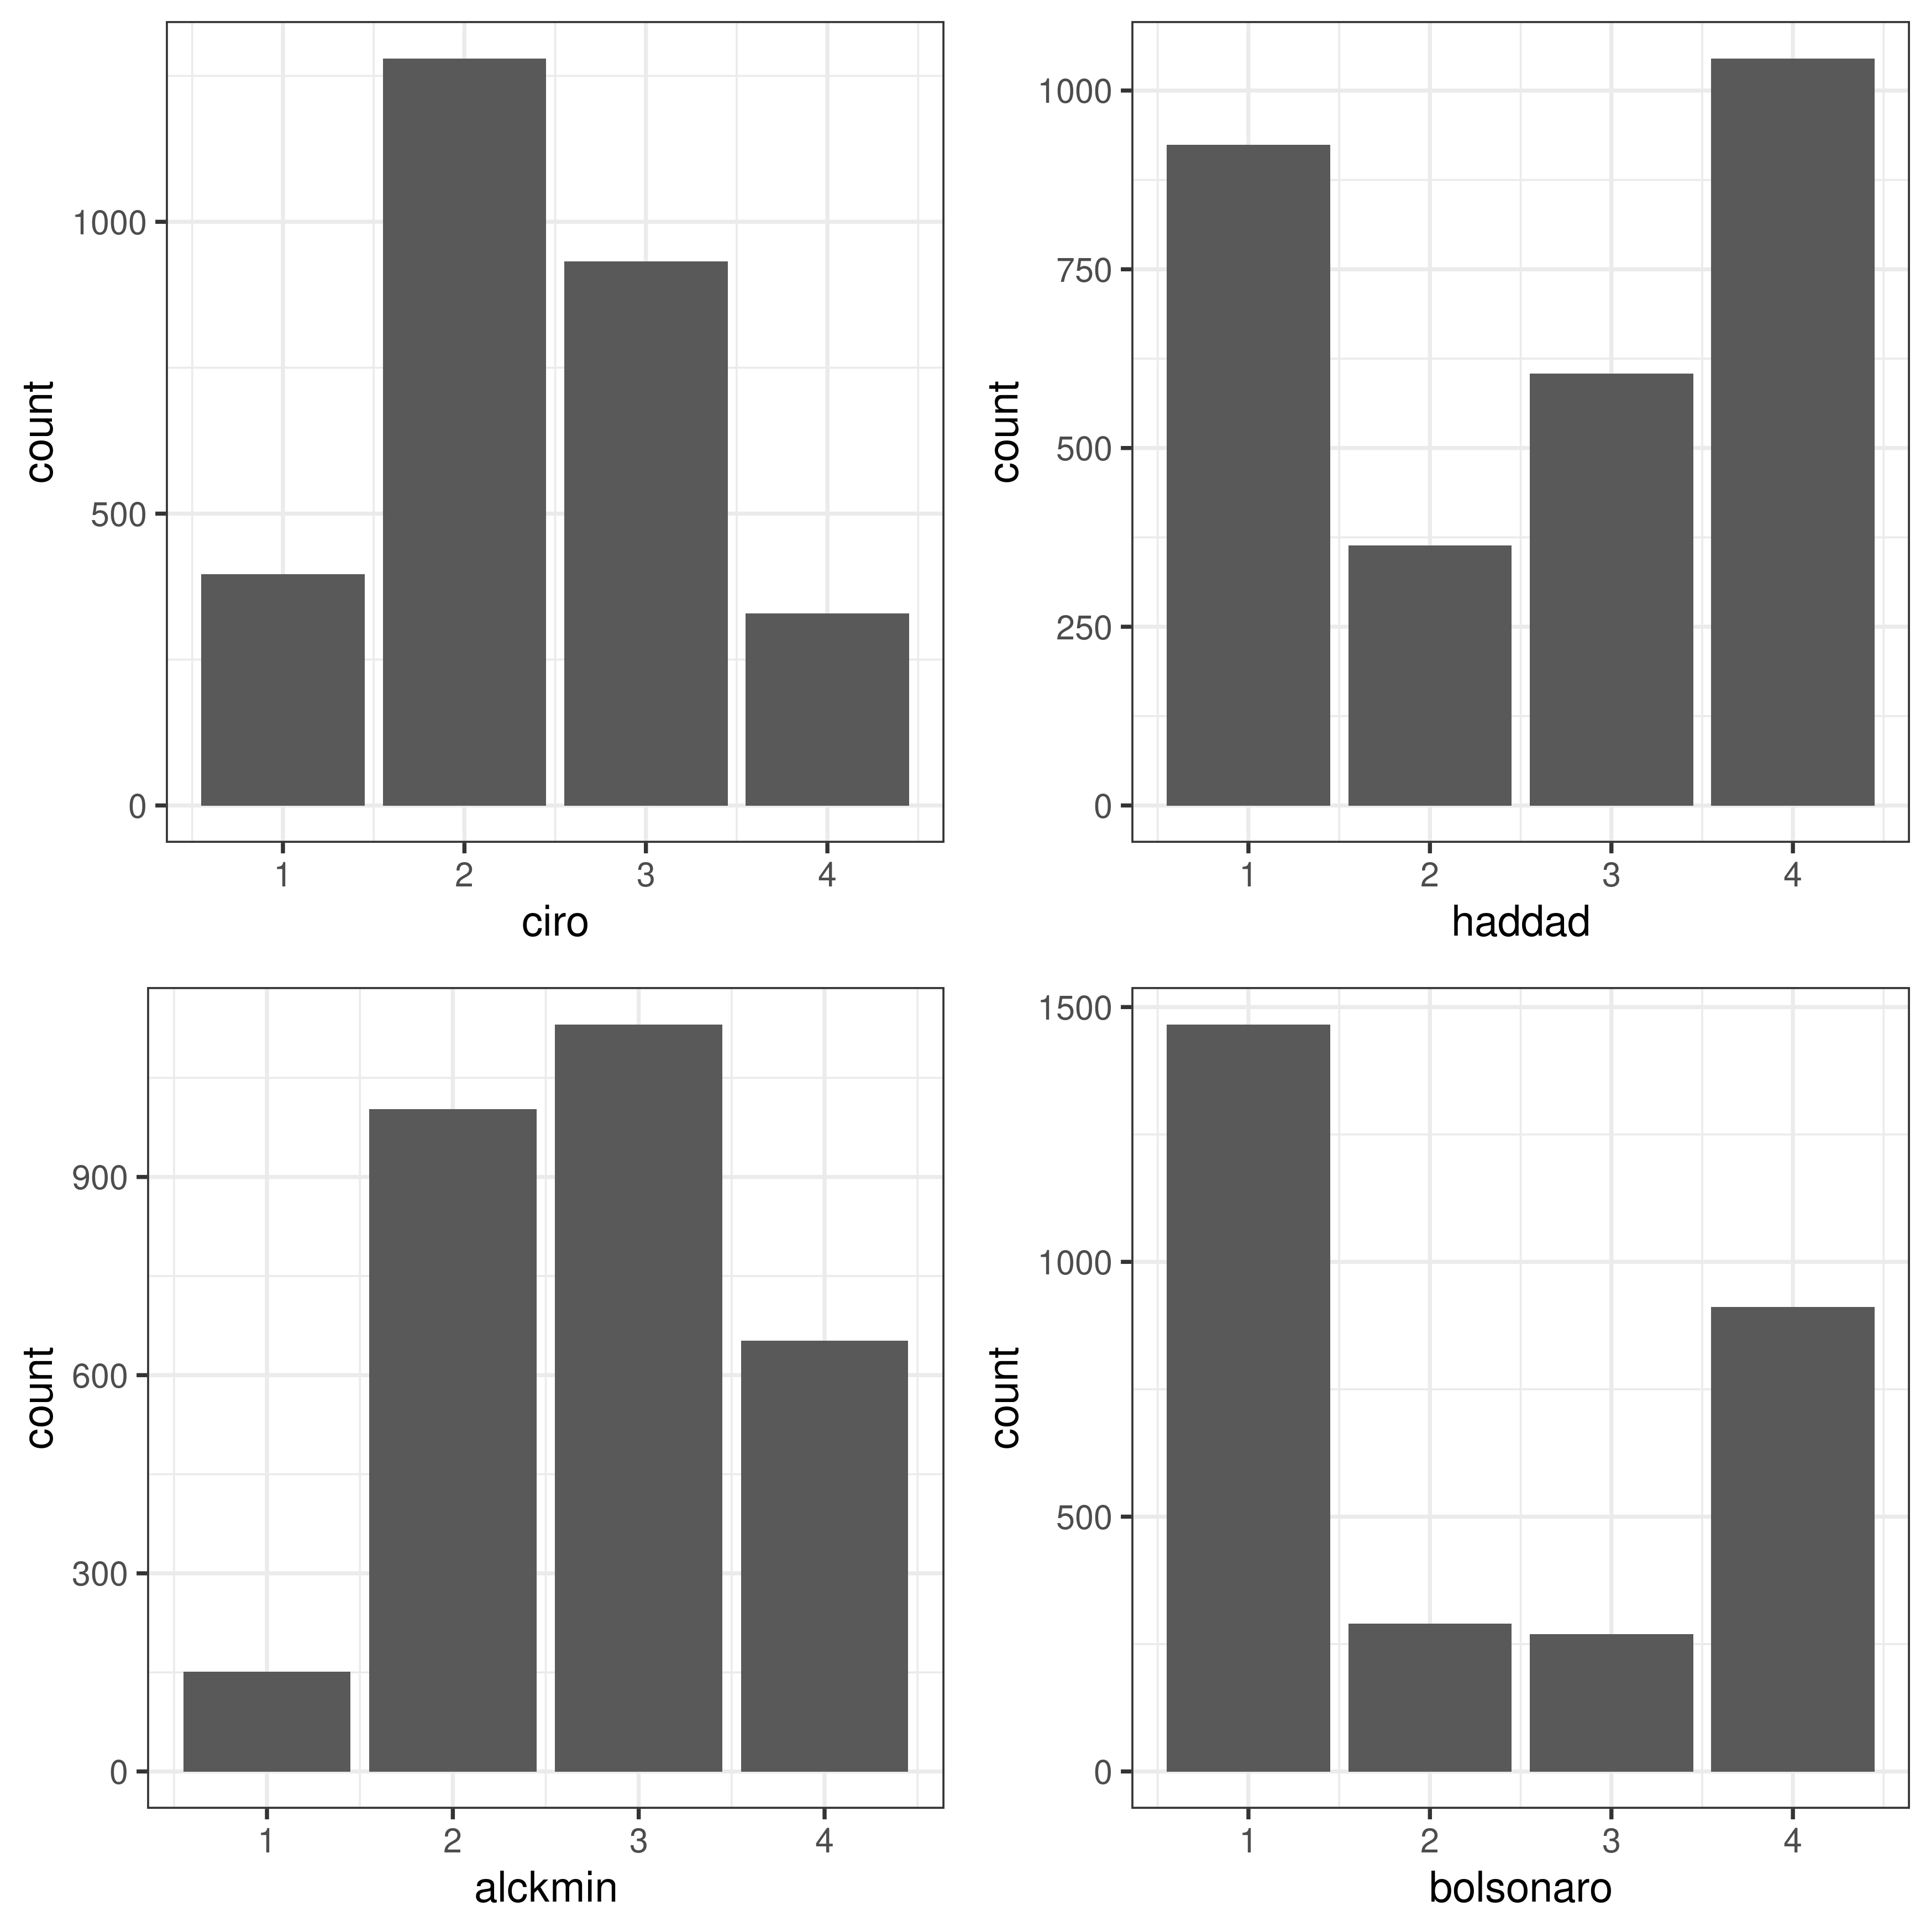
\includegraphics[width=\textwidth]{./images/corrected1_indexes_plot.png}
 \caption{Frequencies at each position}
 \label{fig:counts}
\end{subfigure}
\caption{Transferred Profile}
\label{fig:profile_trans}
\end{figure}

What does this support distribution mean from the point of view of the Borda and
Condorcet procedures? Table \ref{tbl:overallresult} shows what we can infer from
the imputed data. Despite being divisive, Bolsonaro would have won in all
pairwise majority comparisons against any other top candidates. Haddad, however,
would have lost against all others. That is, he was a Condorcet Loser, despite
going to the second round. Ciro who would only have lost against Bolsonaro,
while Alckmin could only win against Haddad. Unlike what was widely believed at
the time and was the motto of his campaign, it is uncertain whether Ciro would
have won against Bolsonaro in a second round. He was not the ``anti-Bolsonaro'',
but merely an ``anti-Haddad'', even more than Bolsonaro. Alckmin, the candidate
with the longest television time and the broadest supporting coalition, would
have lost against Haddad, who was merely a substitute for Lula. However, the
pattern is not reflected in the Borda Scores, which imply the ranking: Ciro >
Bolsonaro > Alckmin > Haddad. Nevertheless, the raw Borda scores of Ciro and
Bolsonaro are actually very similar. If we standardize them we see that the
candidates are practically tied. If we take into account the sampling error,
imputation and transfer degree of freedom, then the most we should conclude is
that the Borda Ranking was Ciro \(\sim\) Bolsonaro > Alckmin > Haddad.

\begin{table}
  \begin{adjustwidth}{3cm}{}
\begin{subtable}[t]{0.48\textwidth}
\centering
          \begin{tabular}{rrrrr}
            &  Alckmin & Bolsonaro & Ciro & Haddad
            \\\hline
            Alckmin & 0.0\% & -12.63\% & -16.99\% & 8.27\% \\
            Bolsonaro & 12.63\% & 0.0\% & 5.48\% & 7.46\% \\
            Ciro & 16.99\% & -5.48\% & 0.0\% & 16.65\% \\
            Haddad & -8.27\% & -7.46\% & -16.65\% & 0.0\% \\\hline
          \end{tabular}
    \caption{Pairwise Margins}
     \label{tbl:margins}
   \end{subtable}
   \vspace*{0.3cm}

\begin{subtable}[t]{0.48\textwidth}
\centering
\begin{tabular}{rrr}
  \hline
 & Borda Score  & Standardized Borda Score\\
  \hline
Alckmin & 7029 & 0.464 \\
  Bolsonaro & 7718 & 0.543 \\
  Ciro & 7756 &  0.547\\
  Haddad & 6867 & 0.446 \\
   \hline
\end{tabular}
\caption{Borda Count Outcome}
\label{tbl:borda}
\end{subtable}
\end{adjustwidth}
\caption{Condorcet and Borda Outcomes}
\label{tbl:overallresult}
\end{table}

The counterfactual analysis can be deeper in the case of positional voting
methods. As discussed in the methods section, with 4 candidates, all results
will lie in the convex hull of three positional voting procedures: plurality,
antiplurality, and vote for two. Note that the score of a candidate will be of
the form \(a + bs_{1} + cs_{2}\), where a is the share it received of votes in
the first position, b in the second, and d in the third position of voters
rankings. Therefore, the scores of each candidate in the inferred ranking for
the 2018 election can be found by assigning values to the equations of Table
~\ref{tbl:ws}. For instance, if we set \(s_{1} = s_{2} = 0\) we recover the
plurality score, after ignoring ``Other'' candidates.

\Big{\textcolor{red}{TODO}} double check this. I think it should be a qs score
\begin{table}
  \begin{tabular}{rr}
    \hline\hline
    \textbf{candidates} & \textbf{w_s tallies} \\
    \texttt{String} & \texttt{SymPy.Sym} \\\hline
    Alckmin & 0.4113*s₁ + 0.4165*s₂ + 0.0514 \\
    Bolsonaro & 0.0392*s₁ + 0.0521*s₂ + 0.4992 \\
    Ciro & 0.4387*s₁ + 0.3612*s₂ + 0.1341 \\
    Haddad & 0.1109*s₁ + 0.1703*s₂ + 0.3154 \\\hline\hline
  \end{tabular}
\end{table}


We can, then, represent the results by an opened tetrahedron, as roughly
depicted in Figure~\ref{fig:ot}. The black downside triangle is the plurality
result, the black downside triangle is antiplurality, the black dot is the vote
for two result and the diamond is the borda count. As expected, the decision
procedures that emphasize the top choice awarded both Bolsonaro and Haddad, to
an extent that the Condorcet loser went to the second round. Note, however, that
Haddad only does well in a small region of the hull. Moreover, we can see that
there are decisional procedures, in which even Alckmin would have beaten both
Bolsonaro and Haddad.

\begin{figure}[H]
 \centering
 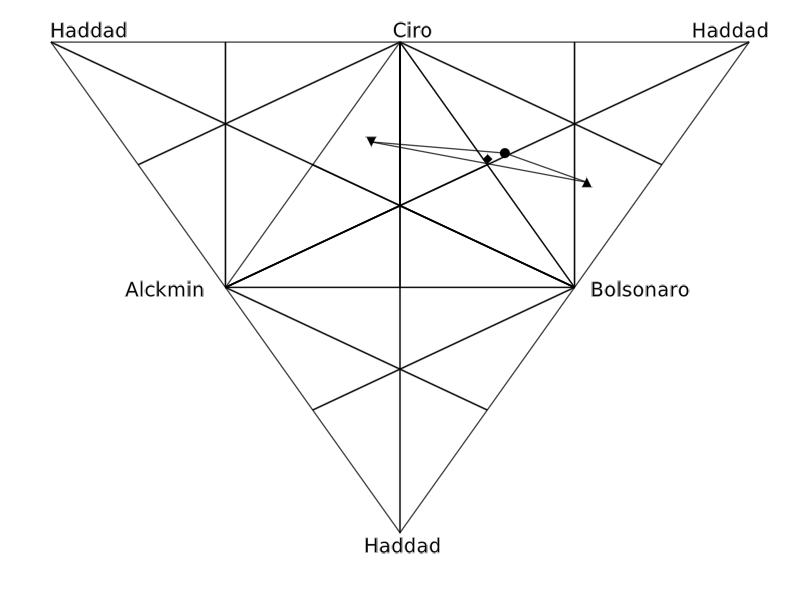
\includegraphics[width=0.8\columnwidth,
 height=0.3\textheight]{./images/opened_tetrahedron1.png}
 \caption{Saari's opened tetrahedron }
 \label{fig:ot}
\end{figure}

But in what precise percentage of the cases would a candidate have beaten
another? Note that by opening the tetrahedron we lose the information provided
by the volume of the subregions of the procedure hull\footnote{Moreover, there
  can be some deformations in my implementation of Figure~\ref{fig:ot}. The
  ensuing percentage computations, however, are exact.}. Nevertheless, algebraic
manipulation of the equations in Table \ref{tbl:ws} allows us to answer this
question. In Table \ref{tbl:ctn} we can se the percentage of scenarios in which
this would have happened. It implies a more complex picture of what happened.
Bolsonaro was the CW, and tied with Ciro as borda winner, however,
he would have won against Ciro in roughly 47\(\%\) of the positional voting
methods. Nevertheless, it shows that, indeed, there were scenarios in which he
would have lost to the more inclusive candidates, Ciro and Alckmin. In Alckmin's
case, this could have happened in surprising \(30\%\) of the cases. However,
Ciro could have beaten him in most,\(\approx 53\%\), of the positional voting
methods. Surprisingly, Haddad, who went to the second round with Bolsonaro,
would never have beaten him. The explanation for that is the following: as shown
in Figure \ref{fig:counts}, Haddad and Bolsonaro were both divisive candidates.
However, Bolsonaro had more support than Haddad. They were not equally
supported/rejected. Given that they were both divisive, most of their support
was in the top choice, they would have fared equally well or badly under the
same positional voting methods, but since Bolsonaro had more first votes and was
less in the bottom of the rankings than Haddad he actually ``positionally
dominated'' Haddad. The same logic applies to another surprising result: Alckmin
would never have beaten Ciro.

\begin{table}[H]
  \centering
  \begin{tabular}{rrrrr}
    \hline
     & Alckmin & Bolsonaro & Ciro & Haddad \\
    \hline
    Alckmin & 0.0 & 0.31 & 0.0 & 0.58 \\
    Bolsonaro & 0.69 & 0.0 & 0.47 & 1.0 \\
    Ciro & 1.0 & 0.53 & 0.0 & 0.81 \\
    Haddad & 0.42 & 0.0 & 0.19 & 0.0 \\\hline\hline
  \end{tabular}
  % \caption{Proportion of victories in the positional voting procedure set}
  \label{tbl:ctn}
\end{table}


Naturally, proportions do not show what, after all, were the decision procedures
in which, for instance, Ciro would have beaten Bolsonaro. Intuitively, voting
procedures that emphasize rejection or more of the middle region of the rankings
should give an advantage to inclusive candidates, which is partially confirmed
by Figure~\ref{fig:ot}. Since the positional voting methods with four candidates
are determined by their \(s_{1}\) and \(s_{2}\) weights, we can visualize all
scenarios by varying them, as in Figure~\ref{fig:positional4c}. It shows the
scenarios Bolsonaro \(\times\) Ciro, Ciro \(\times \) Haddad, and Alckmin
\(\times\) Bolsonaro. Note that, as expected, the only way Alckmin could have
beaten Bolsonaro would be if \(s_{1}\) and \(s_{2}\) were above 0.6. Remember
that when both are 1, the voting procedure is the antiplurality, which is
equivalent to saying which candidate you do not like. However, this universe of
cases was dominated by Ciro, who would have beaten Bolsonaro in any combination
of \(s_{1}\) and \(s_{2}\) higher than the line connecting the points
\((0.51,0.51)\) and \((0.9,0)\). The plot also shows what combinations of
weights lead to \(81\%\)
of Ciro \(>\) Haddad: any combination of weights to the right of the line
segment between \((0.35,0.35)\) and \((0.55,0.0)\).

\begin{figure}[H]
 \centering
 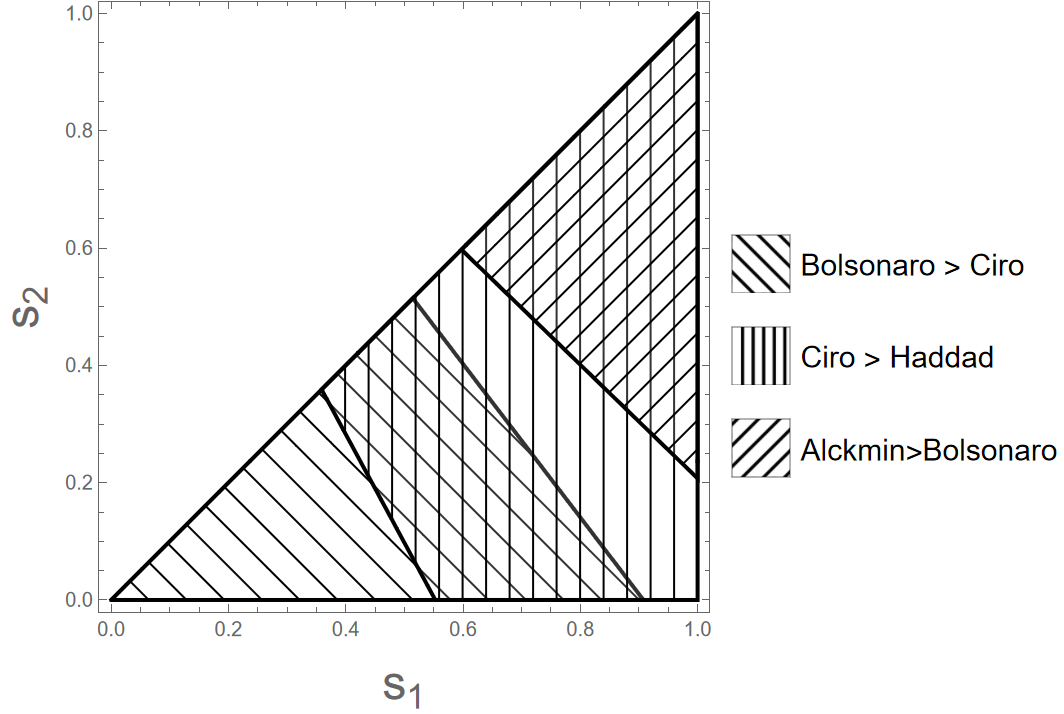
\includegraphics[width=\columnwidth,
 height=0.3\textheight]{./images/counterfactual_triangle.png}
\caption{Victory in terms of values of \(s_{1}\) and \(s_{2}\)}
 \label{fig:positional4c}
\end{figure}

% \begin{table}[]
%     \centering
% \begin{tabular}{|r|r|r|r|}
% \hline
% \textbf{candidates} & \textbf{antiplurality} & \textbf{vote for two} & \textbf{plurality} \\ \hline
% Alckmin             & 0.7779                 & 0.3929                & 0.0514             \\ \hline
% Bolsonaro           & 0.6897                 & 0.5978                & 0.499              \\ \hline
% Ciro                & 0.8879                 & 0.5706                & 0.1348             \\ \hline
% Haddad              & 0.6442                 & 0.4385                & 0.3147             \\ \hline
% \end{tabular}
% \caption{Tallies for boundary positional methods (dropping ``Others'' )}
% \label{tab:positional4c}
% \end{table}

However, neither the CW nor the family of positional voting methods is, in
general, Independent of the Alternative Set \parencite{kaminski2015empirical}.
If we drop or add candidates, the ``social'' ranking might change without
respecting the ordering of the baseline set of alternatives. Consider the
Borda-induced social ranking in this case: Ciro \( \geq \) Bolsonaro > Haddad >
Alckmin. If by dropping Alckmin, the ranking changes to Bolsonaro > Haddad >
Ciro > Alckmin, then the Borda Count, in this case, would be inducing a
``paradoxical.'' result. In Figure ~\ref{fig:c1dropping} we consider alternative
scenarios by dropping one of the top 4 candidates.

The positional voting procedures are eminently well-behaved when dropping
candidates of this dataset. There is a minor tilt towards Bolsonaro winning with
the Borda in Figure~\ref{fig:notah1}, but as I have previously argued this seems
like a tie, given the underlying uncertainty. Notice that in all scenarios where
Bolsonaro is still in the alternative set, he would have been the plurality
winner, though he would have tied with Ciro under Borda, and would have lost
against him with decision procedures that put more weight on rejection, as in
the whole 4 candidates analysis. In the scenario in which Ciro was not in the
set, Bolsonaro would again only have lost against Alckmin, but in a minority of
cases.


   \begin{figure}[H]
        \centering
        \begin{subfigure}[b]{0.475\textwidth}
            \centering
            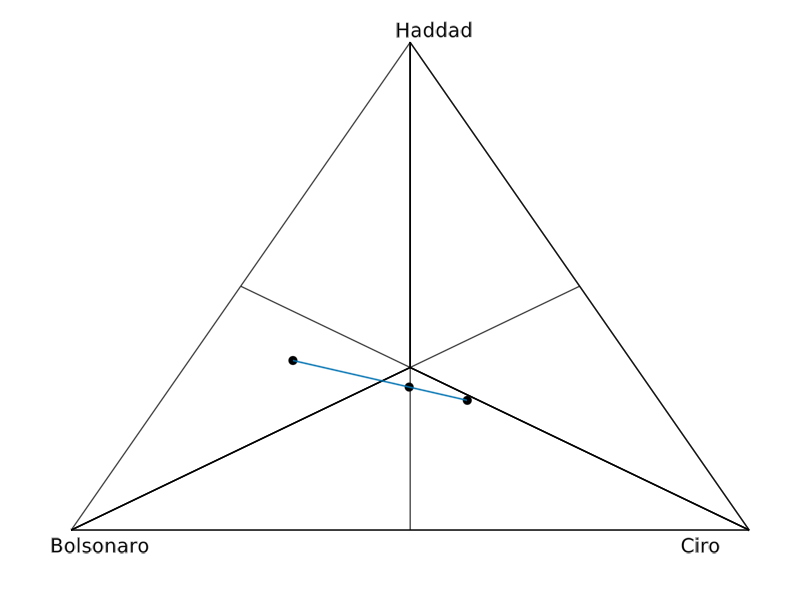
\includegraphics[width=\textwidth]{./images/cw1_nota.png}
             \caption{}%
            % {{\small Network 1}}
            \label{fig:notac1}
        \end{subfigure}
        \hfill
        \begin{subfigure}[b]{0.475\textwidth}
            \centering
            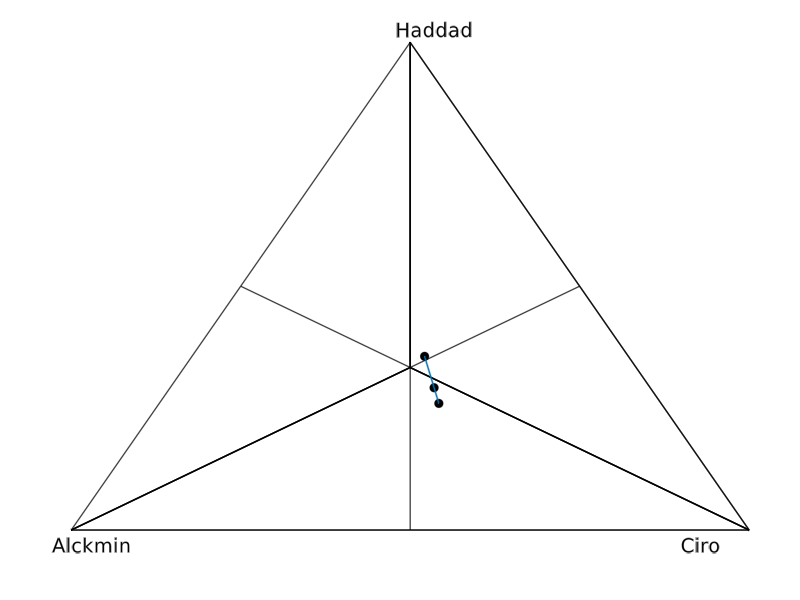
\includegraphics[width=\textwidth]{./images/cw1_notb.png}
             \caption{}%
            % {{\small Network 2}}
            \label{fig:notbc1}
        \end{subfigure}
        \vskip\baselineskip
        \begin{subfigure}[b]{0.475\textwidth}
            \centering
            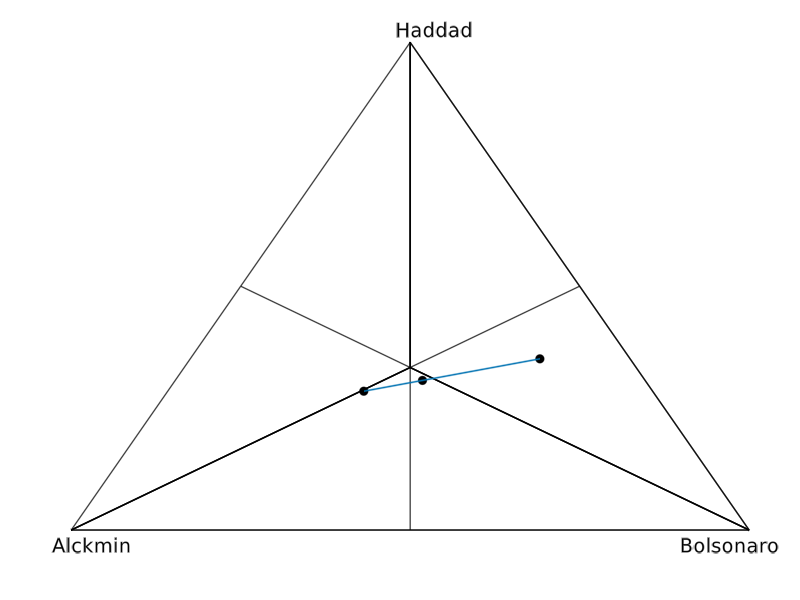
\includegraphics[width=\textwidth]{./images/cw1_notc.png}
            \caption{}%
            \label{fig:notcc1}
        \end{subfigure}
        \hfill
        \begin{subfigure}[b]{0.475\textwidth}
            \centering
            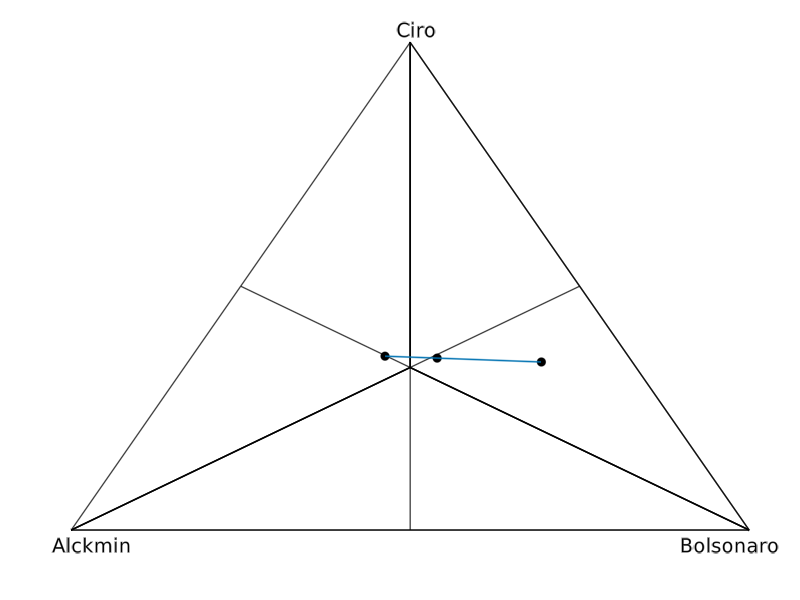
\includegraphics[width=\textwidth]{./images/cw1_noth.png}
             \caption{}%
            % {{\small Network 4}}
            \label{fig:notah1}
        \end{subfigure}
        \caption[  Positional results when dropping one candidate ]
        {\small Positional results after dropping one candidate }
        \label{fig:c1dropping}
    \end{figure}


His victory, thus, was not a fluke or an artifact of institutional technology.
But neither was he a candidate with full positional mandate. This result
revisits the Borda \(\times\) Condorcet controversey. On the one hand, he was
the CW. On the other hand, in the Brazilian case, the
Borda count would have been a stronger barrier against a divisive candidate. As
expected, electoral systems based on just the first positions of citizens'
preferences do ignore, by definition, the distribution of support the
candidates have throughout the whole rankings, and we could expect that divisive
candidates would fared worse under informationally richer decision procedures,
but a divisive candidate can still be a CW with high positional stability. Note
that even though he tied with Ciro in the Borda ranking, he would still have won
in 47\(\%\) of the positional voting methods. Particularly, the ones that
emphasize approval rather than rejection. Moreover, to give \textbf{more} weight
to rejection visavis approval seems unreasonable under any set of normative
expectations demanded of a decision procedure for large scale democratic
elections. The Borda count, due to its symmetry, lies at a threshold: its
constant decrease in assigning weights to the positions in the rankings
guarantees that approval matters more than rejection, but without throwing away
the rejection information. Therefore, highly polarized scenarios can lead to the
election of a divisive candidate which puts in dispute two reasonable metrics of
support: being a CW vs being a BW. All in all, this
means the paper only gives partial support to the hypothesis that
informationally richer decision procedures would be enough to contain divisive
candidates. Two reasonable generalizations of the majoritarian credo conflict
here.

However, Figure~\ref{fig:notbc1} presents an interesting scenario. Here, there
is no conflict between the perspectives: Haddad going to the second round was
purely a institutional fluke. Note that even though Haddad would still be a
plurality winner, the plurality point is close to a tie with Ciro, who
now would have almost 100\(\%\) positional mandate. Moreover, in Table
\ref{tbl:margins} it was shown that Ciro would have beaten him with a majority
pairwise comparison, which gives credence to affirming that Ciro would have won
under a majority with run-off system. In this scenario the most inclusive
candidate would have been elected. Ceteris paribus, it seems the ``only'' way an
agreement between the Borda and Condorcet criteria could be guaranteed to exist
in the Brazilian 2018 case would be if Bolsonaro had never been able to run. In
this scenario, the Condorcet Loser would again be beaten, but now a candidate with a
solid mandate, as endorsed both by the pairwise majority comparisons and
the full hull of positional methods, would have been elected.


\section{Conclusion}

The paper contributes to the analysis of the institutional robustness of
polyarchical systems by considering credible alternative voting procedures
outcomes and properties at a critical juncture in Brazil's political history. We
have demonstrated empirically that Bolsonaro's victory was not merely caused by
the decision procedure, contrary to established theoretical expectations, but
neither was he an undisputed winner under any decision procedure.

In terms of future research, contrasting Haddad with Lula and analyzing the
effect of the knife attack should provide a more comprehensive picture of what
happened in 2018. Moreover, the pipeline for the analysis is highly
reproducible. A similar work can be done to surveys that contain pairwise
comparisons between the top candidates, as many in Brazil do. As such, any other
majoritarian election in Brazil could be analogously analized.

The most glaring limitation of the that paper is that I used only one variable
from the dataset, pairwise comparisons, to simulate alternative scenarios.
However, socio-demographic variables from the dataset could have been used to
strengthen the data imputation procedure. Roughly less than half of the dataset
is constituted of incomplete pairwise comparisons, and there might be valuable
information on the agent's preferences contained in patterns of missingness
\parencite{mcelreath2020statistical}.

Another limitation is that agents adapt to new institutional environments. We
are ignoring strategic voting by assuming a direct translation between
preferences and behavior. However, the percentage of strategic voting in a
large-scale election is an open empirical problem
\parencite{straeten10_strat_sincer_heuris_votin_under,kawai2013inferring}.
Nevertheless, a combination of game-theoretic models with a simulation
parameterized by the inferred ranking distribution is a route of research that
could be pursued.

Though we have analyzed the four top candidates, there can be discrepancies
procedures when we have a subset of the alternatives vs. when we have the whole
set of candidates \parencite{saari2001chaotic}. It is well-known, for instance,
that the Borda Count is susceptible to the winner-turns-loser paradox. This is a
subject for a more thorough analysis. Finally, even though we have analyzed
scenarios in which candidates were removed, it would have been more realistic to
simulate the formation of coalitions and how voters would have reacted to those.
The assumption of a pure additive transfer of votes, implicit when we removed
candidates, is not necessarily valid with coalitions, insofar voters of a
center-left candidate, for instance, could actually vote for the center-right
candidate if they are alienated by an alliance with the Left, which in the case
of the election under scrutiny, was highly rejected, as shown in our analysis.
\printbibliography





\end{document}
